\chapter{基于声音的危险车辆靠近检测}
\section{引言与相关工作}

智能手机已然普及,其功能从最初的通讯设备演变为娱乐设备。越来越多人手机不离手,甚至走路时也在低头用手机,被称为“低头族”。湖南某记者于下班高峰时段仅仅统计了 10 分钟就发现不少于 30 人在走路时低头用手机[1],有人更是低头用手机的同时与抢黄灯的车擦肩而过。南京市因行人走路时低头用手机引起的交通事故每月超过 200 起[2]。由“低头族”引起的车祸数量呈逐年上升趋势[3]。行人低头用手机的行为已经严重影响到了交通安全。


解决“低头族”问题的一个方法是通过立法禁止行人低头使用手机,然而执法难度太大,不具有可行性。如果能够为行人提供一种安全辅助,以警告可能发生的危险,则可以大大减少行人低头看手机引起的事故。行人使用手机容易造成交通事故是因为行人在低头使用手机的过程中眼睛和大脑注意力集中在手机屏幕,听觉和反应力变迟钝[4]。因此,如果需要安全辅助,行人手中的智能手机就是最好的选择。作为一个嵌入了丰富传感器的电子设备,智能手机拥有人的五官一样的感知物理世界的能力[5],用它来帮助行人发现危险再合适不过。


智能手机上有多种传感器可以用来感知汽车靠近的危险[6],例如摄像头。腾讯的产品就推出过用摄像头拍摄的实时内容做聊天背景的功能[7]。Tianyu Wang等人也开发了用摄像头检测车辆靠近手机应用 WalkSafe[8]。然而,此种实现方式不实用。一方面,行人在走路时摄像头是对准的地面,无法感知前后左右的来车。另一方面,摄像头耗电量大[9],在夜间需要开启闪光灯才能使用。最后,人在运动过程中拍摄的内容也会不停颤抖,使用户产生眩晕感,用户体验差。


利用智能手机为行人提供安全辅助并非本文首次提出。Trisha Datta 等人就研究了在城区范围内如何通过手机预测行人可能遇到的潜在危险的方法[20]。他们通过分析用户手机的加速传感器数据,结合城市地图数据,来记录并预测行人的路线,推测出行人可能存在的闯红灯过马路等危险行为。


关于利用声音感知汽车行驶状况的方法也有相关研究。Sergei Astapov 等人通过分析汽车噪声数据实现了车辆经过的检测和分类[21]。汽车经过分为靠近和远离的过程,在这个变化过程中,汽车噪声的频谱能量会出现逐渐增大和逐渐减小的过程。作者通过检测这个变化过程来确定是否有车通过。并从汽车噪声信号提取出频谱特征,用机器学习的方法将其分为A、B两类。该方法需等车辆经过之后才能检测到事件,无法用于危险感知。


\section{基于声音检测的优势及困难}

相比于摄像头,使用麦克风感知汽车靠近的危险是一种更加可行的方式。汽车在行驶的过程中会发出各种噪声[10,11],这为用声音感知汽车靠近提供了理论基础。这种方式存在诸多优点:1)当行人的注意力被吸引到手机屏幕,从而对这些声音反应迟钝时,手机的麦克风依然对声音敏感。2)麦克风收集到的声音数据来自于空间的各个方向,其感知空间要远大于摄像头。3)整个感知过程全部后台完成,不存在让用户产生眩晕的情况。4)手机麦克风感知到的声音频谱[12]宽于人类耳朵所能听到的频谱[13],从这个意义上来说,手机麦克风的感知能力要强于人耳。


利用智能手机麦克风感知危险虽然有很多优势,也存在诸多挑战。1)必须在只依靠手机的情况下,感知用户的行走状态以及所处环境。 2)汽车噪声信号成分复杂[14],从中提取信息十分困难。3)危险检测系统对即时性要求高,而智能手机计算能力有限,复杂算法无法直接应用。



\section{车辆噪声分析}

\subsection{音频处理方法}
本文采用智能手机内置麦克风收集的PCM原始语音数据[22]为数据源,通过对声音数据的预处理和特征分析找到与汽车靠近有关的信息。本小节对文中用到的语音处理方法予以说明。

\subsubsection{改进的音量计算}
音量的客观评价尺度是声音的振幅大小,传统音量计算以分贝(dBm)为单位。事实上,分贝的大小反应了人耳对声音大小的感受,与真实振幅不是线性关系[23]。分贝计算过程包含对数计算,为了减少计算量本文采用简化的音量计算方式。对一段时间长度为,共有$N$ 个采样点的时域信号,其音量的计算方法为:

\begin{equation}
\label{equ:chap3:volume}
V_{\Delta t}= \frac{\sum_{m=0}^{N-1}\left | x\left ( m \right ) \right |}{N}
\end{equation}

\subsubsection{快速傅里叶变换}
音频的频域特征是由时域上的信号分解得到,这一分解过程即是傅里叶变换(Fourier Transform, FT)。对于时域上离散的音频信号,采用离散傅里叶变换进行分解(Discrete Fourier Transform,DFT)。对于一段有限的离散信号$x(m)$,其长度为$N$,则 DFT 公式为:

\begin{equation}
\label{equ:chap3:dft}
X\left( k \right) = \sum\limits_{m = 0}^{N - 1} {x\left( m \right){e^{ - j{\textstyle{{2\pi } \over N}}mk}},k = 0,...,N - 1}
\end{equation}


公式~\ref{equ:chap3:dft}中有两个整型变量:$m$和$k$。其计算复杂性为,为了减小计算复杂性,快速傅里叶变换(Fast Fourier Transforms, FFT)应运而生。本文中使用的 FFT 版本为 MIT 研究员实现的 FFTW[24]。

\subsubsection{滤波}

汽车噪声的成分复杂,在提取其周期性的过程中,本文用Savitzky Golay (SG) 滤波器对信号进行了滤波。SG 滤波器被广泛地运用于数据的平滑除噪,是一种在时域上基于局域多项式最小二乘法拟合的滤波方法。该滤波器最大的特点在于其滤除噪声的同时可以保持信号的形状和宽度不变。

\subsection{汽笛声的检测}

当系统检测到瞬时增大的音量后,会先判断是否为汽车笛声。汽车笛声为中心频率在 800 Hz左右的声源,且随着汽车靠近其中心频率会有小幅升高。

\subsection{车辆噪声音量变化属性}

汽车行驶中发动机会产生噪声,轮胎和地面摩擦会产生噪声,车身震动会产生噪声。因此,当车辆靠近时,必然会引起音量增大。当系统检测到音量渐渐增大,便可能是有汽车正在靠近。


如图~\ref{fig:volume}(a)所示,汽车靠近的过程中,噪声音量缓慢呈增大的趋势。相比而言,人声等常见噪声一般具有瞬时发生的特性,其引起的音量变化也会反映出瞬时发生的特点如图~\ref{fig:volume}(b)所示。汽车引发的音量变化斜率低,非汽车引发的音量变化斜率高,通过这一特性可以快速排除明显的非汽车噪声。对于疑似的汽车噪声,则尝试进行周期性提取和频谱特征曲线的分析。

\begin{figure}[htbp] % use float package if you want it here
  \centering
  \includegraphics[width=4in]{volume}
  \caption[音量变化特性对比]{人声与汽车靠近噪声音量变化对比}
  \label{fig:volume}
\end{figure}


\subsection{车辆噪声周期性提取}

汽车在行驶过程中的噪声主要由发动机和路面产生的摩擦产生,具有周期性.作者通过对疑似车辆靠近产生的噪声信号进行滤波处理,去除了干扰,从中提取出了噪声中隐藏的周期性,并分析出了汽车靠近过程独有的频率变化特性.

\subsubsection{音频周期提取方法简介}

提取音频信号周期频率最简单的方式是将其可视化,即画出信号随时间变化的波形图,然后用肉眼去观察波形的变化周期。实际的处理中,这种方法明显不具有可行性,本文需要的是一种可以让程序自动快速提取周期的方式。于是本文借鉴了音频处理中的一种成熟技术,音高追踪。

音高追踪是音频处理的一种成熟技术,是音频领域进行更复杂任务的第一步。研究员们已经在该技术上进行了长达几十年的研究,人们对其原理了解透彻。经过相关调研,作者发现该技术可以很好的用在汽车噪音的周期性提取上。

提取周期可选的技术有基于时域的 Auto Correlation Function(ACF)、Normalized Squared Difference Function(NSDF)、Average Magnitude Difference Function(AMDF)和基于频域的 Harmonic Product Spectrum(HPS)、倒频谱共五种方式。经过筛选与实验,本文最终选择了 ACF。

ACF 是基于时域的方法,它的本质是计算一段信号$s(i),i=0,...,n-1$和其延时信号之间的相似性,其计算公式如下:

\begin{equation}
\label{equ:chap3:acf}
ACF\left( \tau  \right) = \sum\limits_{i = 0}^{n - 1 - \tau } {s\left( i \right)s\left( {i + \tau } \right)} 
\end{equation}


公式~\ref{equ:chap3:acf}中的$\tau$代表时间上的步长,其单位是样本点的个数。音频信号$s(i)$的一个周期所包含的样本个数即是使得函数$acf(\tau)$取最大值的$\tau$,如图~\ref{fig:acf}所示。


\begin{figure}[htbp] % use float package if you want it here
  \centering
  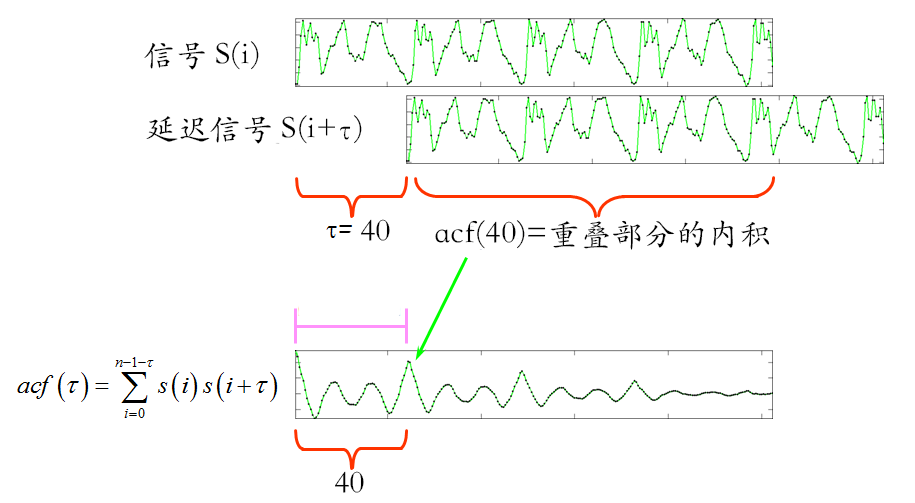
\includegraphics[width=5in]{acf}
  \caption{音频周期提取示意图}
  \label{fig:acf}
\end{figure}



\subsubsection{车辆噪声周期提取过程}

与普通音频可以直接使用ACF算法追踪音高不同的是,汽车的噪音成分十分复杂,直接使用ACF算法是没有效果的,必须要先进行预处理。其预处理及提取周期的基本过程如下:

\begin{compactenum}
\item 用SG滤波器对信号进行滤波。

\item 将滤波后的信号切分为$30ms$左右的帧,相邻帧之间可以有重叠。

\item 计算每个帧的周期频率,如图~\ref{fig:findpeak} 所示。

\item 过滤掉严重偏离限定范围的周期频率。

\item 对整段音频周期频率进行平滑。

\end{compactenum}

\begin{figure}[htbp] % use float package if you want it here
  \centering
  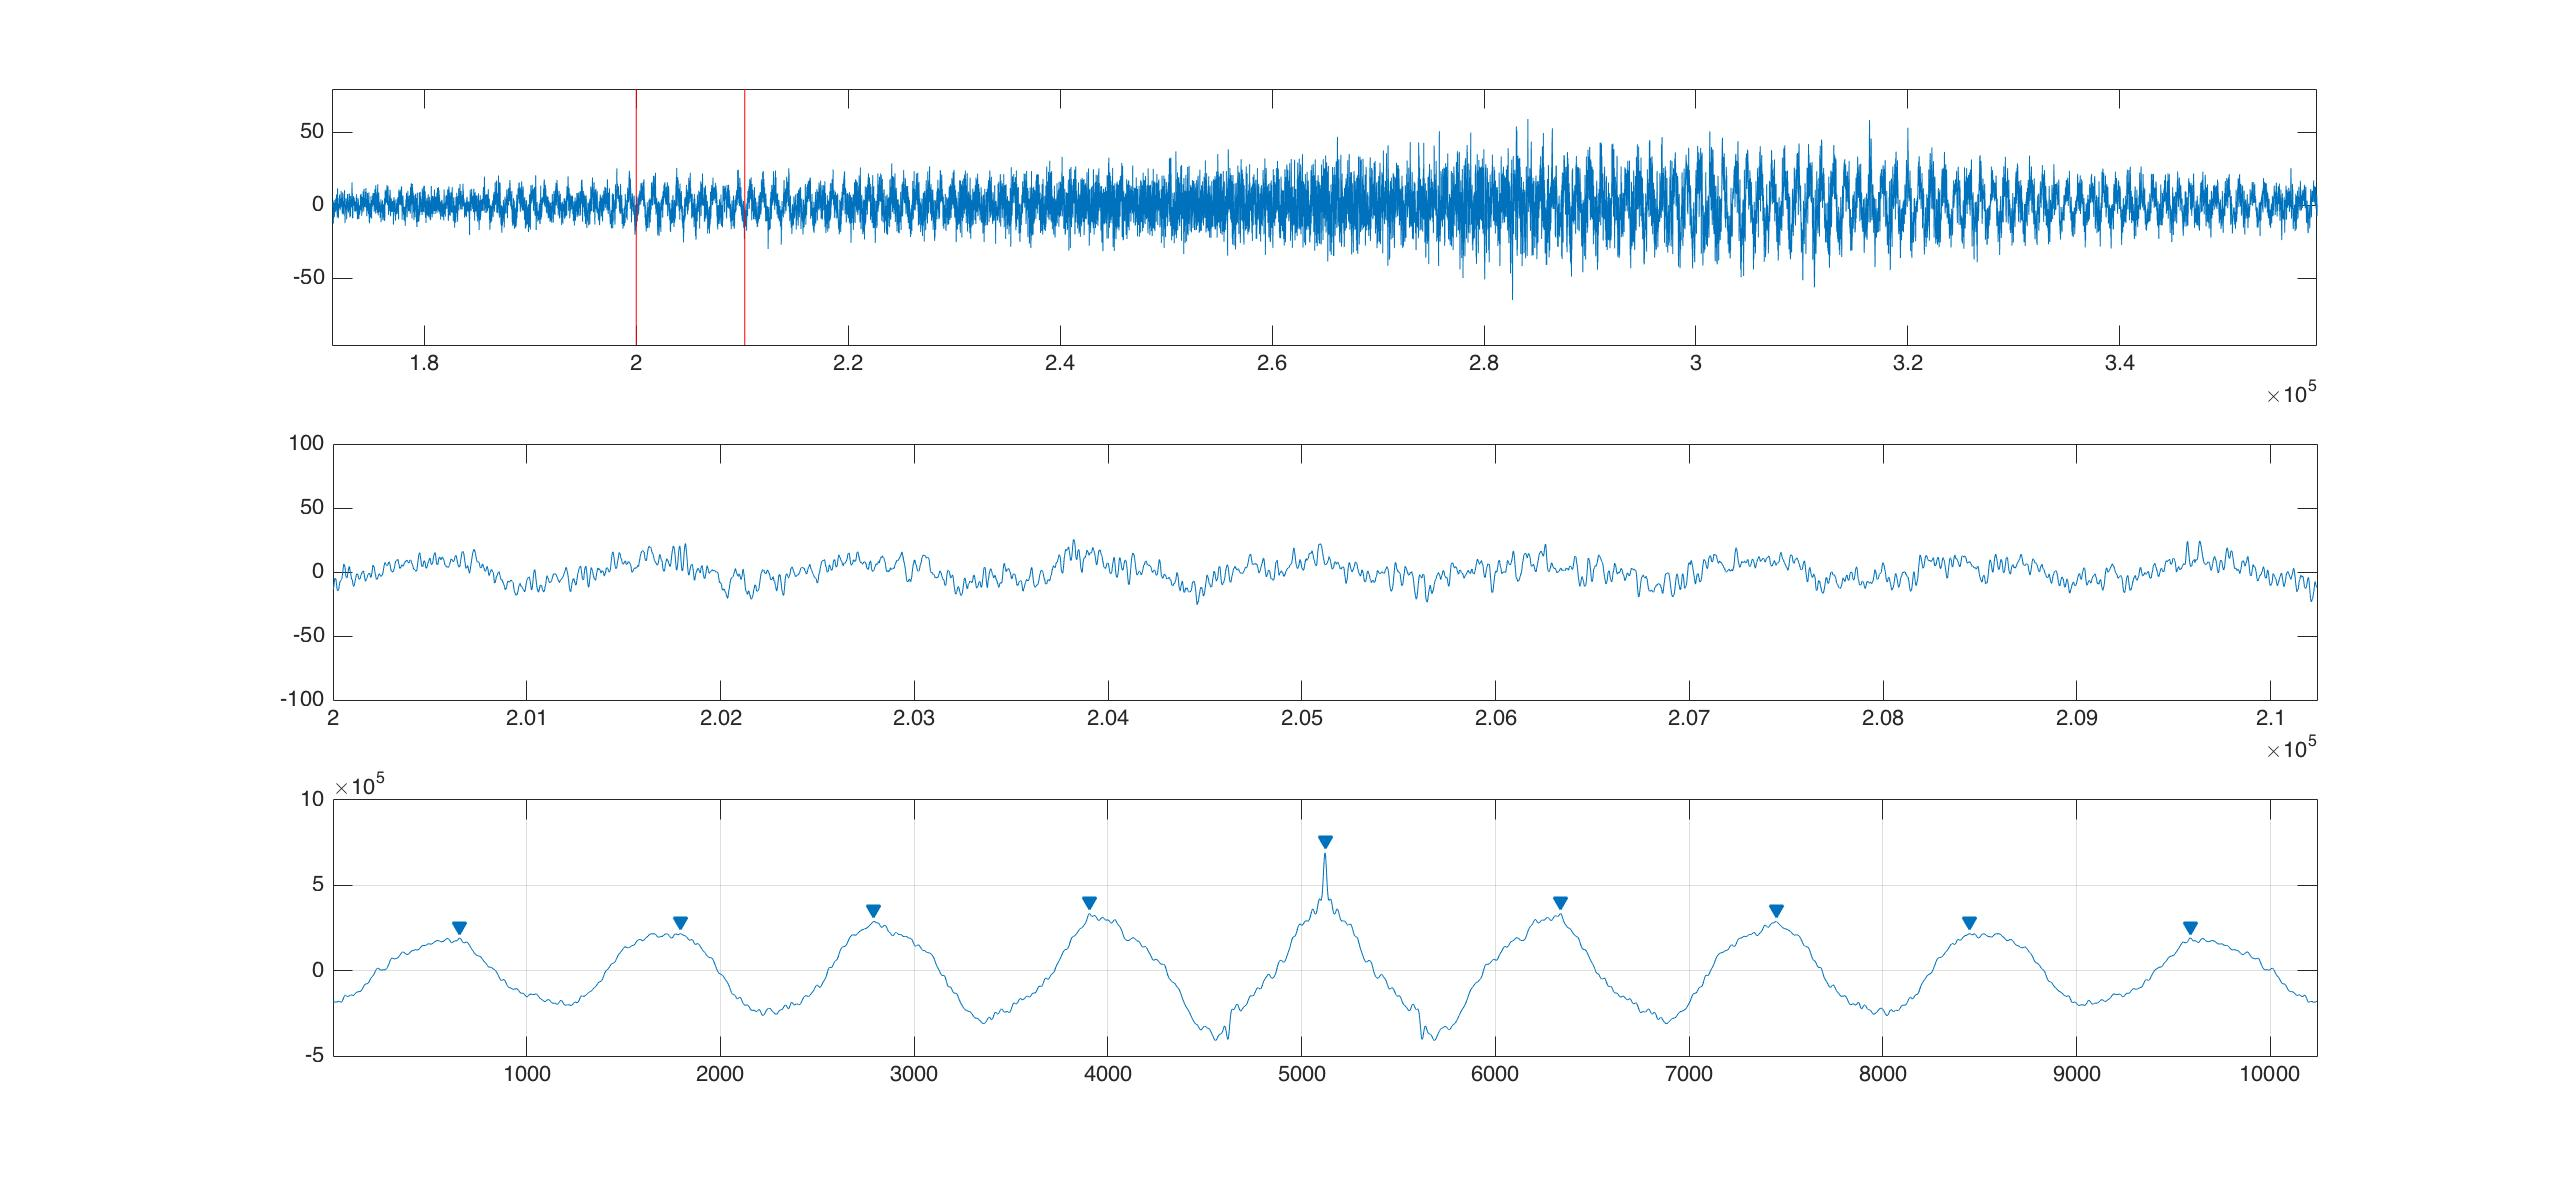
\includegraphics[width=5in]{findpeak}
  \caption{音频周期提取示意图}
  \label{fig:findpeak}
\end{figure}



\subsubsection{周期提取过程结果}

以一辆速度为 25km/h 行驶的小汽车为例,从其产生的噪声中可以提取出较稳定的周期性,如图~\ref{fig:cycle}(a)所示.且随着汽车靠近,提取到的频率呈小幅度增加的趋势,如图~\ref{fig:cycle}(b)所示. 

\begin{figure}[htbp] % use float package if you want it here
  \centering
  \includegraphics[width=6in]{cycle}
  \caption[音量变化特性对比]{人声与汽车靠近噪声音量变化对比}
  \label{fig:cycle}
\end{figure}



\subsection{车辆噪声频谱}

\subsubsection{车辆噪声成分分析}
不同于常见乐器、歌声等声源只在特定频段分布有能量,汽车噪声的频谱分布在几Hz到几千Hz的极宽频段上。汽车噪声主要由三部分组成:汽车轮胎和地面的声音、汽车发动机产生的声音和汽车外壳震动产生的声音。

为了增大汽车轮胎相对于路面的摩擦力,汽车轮胎都会设计各种各样的花纹,如图~\ref{fig:huawen}所示。在汽车行驶的过程中,花纹间隙中的空气会随着车轮与地面的接触而遭到挤压,从而发出噼啪的声音。合理的设计轮胎花纹可以有效降低噪声,但是无法彻底消除。

发动机产生噪声在汽车整车噪声中占较大的比重,发动机内部液体的燃烧,排气进气以及风扇的转动,还有内部零件在机械振动下的摩擦碰撞都是其产生噪音的原因。

汽车外壳会产生噪音主要是由发动机的振动和路面的不平整导致,另外随着汽车的老化,外壳部件之间的加固慢慢变松,外壳碰撞加剧,噪声也会更大。

\begin{figure}[htbp] % use float package if you want it here
  \centering
  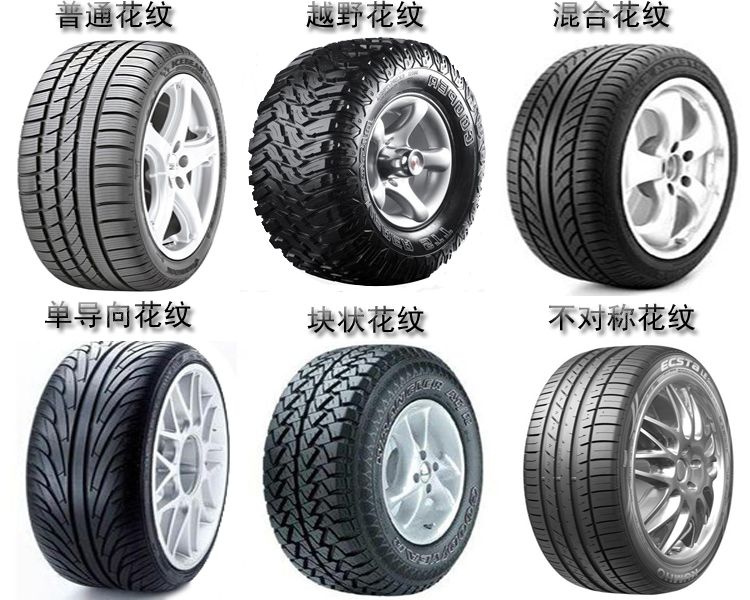
\includegraphics[width=3in]{huawen}
  \caption{汽车轮胎花纹}
  \label{fig:huawen}
\end{figure}




\subsubsection{车辆噪声频谱特征曲线}
虽然相比常见声源,汽车噪声成分复杂,但经实验发现汽车噪声频谱具有明显特征,且该特征为市面上大部分汽车共有。通过频谱特征曲线可有效区分汽车噪声和非汽车噪声。图~\ref{fig:frequencyCompare}所示即为一典型汽车噪声样本和一普通噪声样本的频谱特征曲线对比,其中~\ref{fig:frequencyCompare}(a)为汽车噪声频谱, ~\ref{fig:frequencyCompare}(b)为其特征曲线, ~\ref{fig:frequencyCompare}(c)人声频谱, ~\ref{fig:frequencyCompare}(d)为其特征曲线。


\begin{figure}[htbp] % use float package if you want it here
  \centering
  \includegraphics[width=5in]{frequencyCompare}
  \caption{人声与汽车噪声频谱对比}
  \label{fig:frequencyCompare}
\end{figure}

本文用200个标注样本计算出了汽车噪声基准频谱特征曲线,如图~\ref{fig:frequencyLine}所示。通过计算待测样本的频谱特征曲线和基准频谱特征曲线的相似性即可推测声音来自于汽车的可能性。当两者相似性大于某个阈值时,推测样本为汽车噪声,本文中阈值取$TH=0.95$。

\begin{figure}[htbp] % use float package if you want it here
  \centering
  \includegraphics[width=3in]{frequencyLine}
  \caption{汽车噪声频谱特征曲线}
  \label{fig:frequencyLine}
\end{figure}


\section{基于K近邻算法的分类}

通过对车辆噪声进行简单的时频分析,我们可以快速的排除干扰样本,鉴别出大部分汽车靠近事件。但经实验发现,仍有部分汽车靠近事件被漏报。这部分样本多表现为无法提取明显周期性或者特征曲线和基准特征曲线差异较大。多次实践后,我们最终成功利用K近邻算法对这部分样本进行分类。

\subsection{KNN算法原理及优势}

K近邻算法(K Nearest Neighbor)是机器学习领域一种基本的算法。它原理简单,功能强大,既可以用于分类也可以用于回归。本文中只应用其做分类,即将一个收集到的音频样本分汽车靠近和非汽车靠近两类。在K近邻算法中,目标样本最终属于哪一类由与其距离最近的$K$个邻居决定。即离目标样本最近的$K$个邻居中,包含哪一类样本个数最多,目标样本就被分到哪一类。$K$值选取的不同,会影响分类的结果,如图~\ref{fig:knn}所示,当$K$值取3时和$K$值取5时,目标样本会被分到两种不同的种类。


\begin{figure}[htbp] % use float package if you want it here
  \centering
  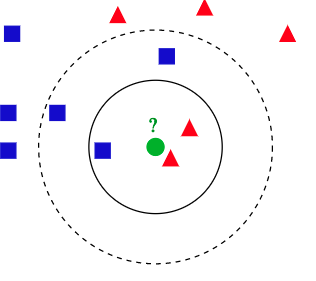
\includegraphics[width=3in]{knn}
  \caption{参数K对分类结果的影响}
  \label{fig:knn}
\end{figure}


用来表征两个样本间距离方式有很多种,通常有欧氏距离、马氏距离、余弦相似性等。本文采用的余弦相似性来表征两个样本的距离,用$A$和$B$来表示两个样本的特征向量,则两者间的距离可由公式~\ref{equ:chap3:similarity}计算得出:

\begin{equation}
\label{equ:chap3:similarity}
{D_{A,B}} = \cos \left( \theta  \right) = \frac{{A \bullet B}}{{\left\| A \right\|\left\| B \right\|}} = \frac{{\sum\limits_{i = 1}^n {{A_i} \times {B_i}} }}{{\sqrt {\sum\limits_{i = 1}^n {{{\left( {{A_i}} \right)}^2}} } \sqrt {\sum\limits_{i = 1}^n {{{\left( {{B_i}} \right)}^2}} } }}
\end{equation}


K近邻算法的优势在于其基本不需要训练,且即使样本量少或者样本不具有明显可分性时也可达到很好的效果。本文中,属于非汽车靠近事件的样本差异较大,且占样本的比例较小。因此在样本可分性低的情况下,我们选择了K近邻算法。

\subsection{分类特征选取}
分类用到的特征为只与当前信号帧有关的瞬时特征。它们可以很好地反映信号的波动特性,区分不同的信号。对一段长度为$K$的频谱信号$X(k)$提取以下四种特征:

\begin{compactenum}
\item 频带能量。频带能量反应了第$i$个频带上的能量特性。其计算方法如公式~\ref{equ:chap3:bandenergy}所示。

\begin{equation}
\label{equ:chap3:bandenergy}
{X_{be}}\left( i \right) = \frac{{\sum\limits_{l \in {S_i}} {{{\left| {{X_t}\left( l \right)} \right|}^2}} }}{{\sum\limits_{k = 1}^K {{{\left| {{X_t}\left( k \right)} \right|}^2}} }}
\end{equation}
公式~\ref{equ:chap3:bandenergy}中$S_i$表示所有在$i$频带的频谱样本集合。频带按照梅尔刻度(Mel scale)进行划分。梅尔刻度是一种基于人耳对等距音高变化的感官判断而定的非线性频率刻度,其计算方法如公式~\ref{equ:chap3:mel}所示:

\begin{equation}
\label{equ:chap3:mel}
Mel\left( f \right) = 2595 \cdot \log \left( {1 + \frac{f}{{700}}} \right)
\end{equation}


\item 频谱重心。该指标用于反映信号频率的重心分布情况。计算方法如公式~\ref{equ:chap3:signalcenter}所示。

\begin{equation}
\label{equ:chap3:signalcenter}
{X_{sc}} = \frac{{\sum\limits_{k = 1}^K {k \cdot \left| {{X_t}\left( k \right)} \right|} }}{{\sum\limits_{k = 1}^K {\left| {{X_t}\left( k \right)} \right|} }}
\end{equation}

\item 频谱衰减。它可以反映出占总能量一定比重的能量集中在哪个频率一下。该比重由阈值$TH$指定,$TH \in \left[ {0,1} \right]$,本文取$TH = 0.8$。其计算方法如公式~\ref{equ:chap3:signalredution}所示。


\begin{equation}
\label{equ:chap3:signalredution}
{X_{sr}} = \arg {\max _p}\left[ {\sum\limits_{l = 1}^p {{{\left| {{X_t}\left( l \right)} \right|}^2} \le TH \cdot \sum\limits_{k = 1}^K {\left| {{X_t}{{\left( k \right)}^2}} \right|} } } \right]
\end{equation}

\item 频谱斜率。频谱斜率反映了音频信号由低频到高频方向的衰减趋势。其计算方式是对频谱样本进行线性回归,拟合成一维直线。一维直线由斜率和直线与$y$ 轴的交点指定。斜率的计算方法如公式~\ref{equ:chap3:xielv}所示。

\begin{equation}
\label{equ:chap3:xielv}
a = \frac{{K\sum\limits_{k = 1}^K {k \cdot \left| {{X_t}\left( k \right)} \right| - \sum\limits_{k = 1}^K {k\sum\limits_{k = 1}^K {\left| {{X_t}\left( k \right)} \right|} } } }}{{K\sum\limits_{k = 1}^K {{k^2} - {{\left( {\sum\limits_{k = 1}^K k } \right)}^2}} }}
\end{equation}

直线与$y$轴交点的计算方法如公式~\ref{equ:chap3:jiaodian}所示。

\begin{equation}
\label{equ:chap3:jiaodian}
b = \frac{{\sum\limits_{k = 1}^K {k \cdot \left| {{X_t}\left( k \right)} \right|\sum\limits_{k = 1}^K {{k^2}}  - \sum\limits_{k = 1}^K {k\sum\limits_{k = 1}^K {k \cdot \left| {{X_t}\left( k \right)} \right|} } } }}{{K\sum\limits_{k = 1}^K {{k^2} - {{\left( {\sum\limits_{k = 1}^K k } \right)}^2}} }}
\end{equation}

\end{compactenum}


\subsection{分类效果}

我们选取200个汽车靠近样本和200个非汽车靠近样本,共进行10次循环交叉验证,每次随机抽取60个汽车靠近样本和60个非汽车靠近的样本组成交叉验证集。结果表明,本应用中K近邻算法中$k = 9$时,算法达到最好效果。其识别结果平均值如表~\ref{table:knn}所示。

\begin{table}[htb]
  \centering
  \caption{K近邻算法分类结果}
  \label{table:knn}
  \begin{tabularx}{0.9\linewidth}{ccc}
  \toprule
  &{\hei 汽车靠近样本} & {\hei 非汽车靠近样本} \\
  \midrule
  被识别为汽车靠近 & 96.33\% & 5.17\% \\
  被识别为非汽车靠近 & 3.67\% & 94.83\% \\
  \bottomrule
  \end{tabularx}
\end{table}



\section{系统设计}

\subsection{系统架构}

如上文所述,基于智能手机麦克风可感知到汽车靠近有关的信息。但真正将此方法应用到智能手机还存在诸多限制。一方面,检测汽车靠近的目的是防止用户发生车祸,当汽车靠近时,系统必须在尽可能短的时间内响应,从而给用户留出躲避车辆的反应时间。另一方面,智能手机电量和计算能力有限,麦克风长时开启会损耗电量,太过复杂的算法会降低系统反应速度。考虑到性能和资源的矛盾,我们设计了一个具有三个模块的感知系统架构:用户行为感知、音频轻量特征分析和音频复杂特征分析,用户行为感知模块分析用户状态,决定麦克风及其余两个模块是否开启,以减小能耗。轻量特征分析模块主要进行时域分析,其计算量小,利于快速反应,但是容易受到干扰。复杂特征分析模块主要进行频域分析,其抗干扰性强,但计算量较大,用于处理前者无法区分的数据。其系统架构如图~\ref{fig:design}所示,工作流程如图~\ref{fig:workflow}所示。

\begin{figure}[htbp] % use float package if you want it here
  \centering
  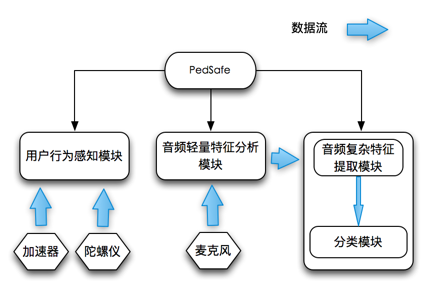
\includegraphics[width=4in]{pedsafeStructure}
  \caption{车辆靠近感知系统架构如图}
  \label{fig:design}
\end{figure}

\begin{figure}[htbp] % use float package if you want it here
  \centering
  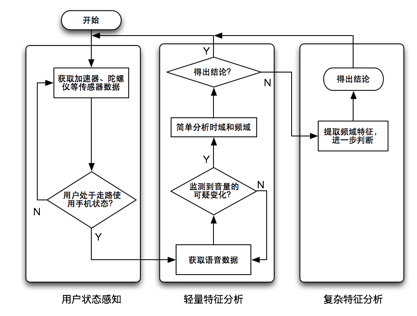
\includegraphics[width=4in]{pedsafeWorkflow}
  \caption{车辆靠近感知工作流程图}
  \label{fig:workflow}
\end{figure}


\subsection{数据获取}
感知车辆靠近事件主要用到了手机的麦克风,加速器,陀螺仪和GPS数据。本文中我们基于Android系统开发Demo应用获取这些数据。获取这些数据的大致步骤如下:
\begin{compactenum}
\item 申请麦克风,加速器,陀螺仪和GPS对应的权限。
\item 实现对应接口类。
\item 初始化采样率,数据格式等参数。
\item 启动相关服务服务,获取数据。
\item 关闭服务,结束获取数据。
\end{compactenum}


各设备对应的权限、涉及的主要API对应列表如~\ref{tab:androidApi}所示。

\begin{table}[htb]
\centering
\caption{获取设备数据所需权限及API列表}
\label{tab:androidApi}
\begin{tabularx}{0.9\linewidth}{ccc}
\toprule
& {\hei 所需权限} & {\hei 相关API} \\
\midrule
麦克风 & android.permission.RECORD\_AUDIO & AudioRecord \\
加速器 & android.permission.SENSOR\_ENABLE & SensorManager \\
陀螺仪 & android.permission.SENSOR\_ENABLE & SensorManager \\
GPS & android.permission.ACCESS\_FINE\_LOCATION & LocationManager \\
\bottomrule
\end{tabularx}
\end{table}


\subsection{用户行走状态分析模块}

麦克风于智能手机是较高耗电器件[9]。增加一个低能耗的用户状态感知模块可以缓解能耗问题。该模块检测用户状态,确保只有用户处于边走路边使用手机的状态时,麦克风才被唤醒。该模块通过分析加速传感器和陀螺仪的数据推测用户状态。

(1)	加速传感器

加速传感器可以监测手机任意时刻的在$x、y、z$方向上的加速度,坐标轴的方向如~\ref{fig:accelerator}所示,其测量原理是惯性。加速传感器已被广泛应用于计步器、导航、定位等应用。利用加速传感器感知用户的行走状态的技术已成熟[3]。

\begin{figure}[htbp] % use float package if you want it here
  \centering
  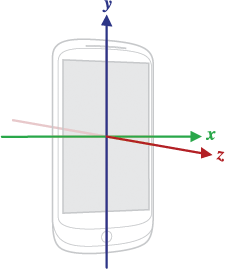
\includegraphics[width=2in]{accelerator}
  \caption{传感器坐标示意图}
  \label{fig:accelerator}
\end{figure}



(2)	陀螺仪

陀螺仪可以准确的测量手机在各方向上的转动,例如,当用户手机横屏,屏幕的内容也会随之转换方向,这个过程的检测主要有陀螺仪完成。同样的,当用户处于使用手机的状态时,手机屏幕处于向上状态,陀螺仪可以检测到此状态。

(3) 位置

位置数据指通过手机自带的GPS或者运营商提供的网络位置数据。位置数据可以帮助我们判断用户是否是在户外。


本文引用并改进了Zhengjuan Zhou[3] 的用户行为识别算法,根据加速器数据推测用户的行走状态,陀螺仪数据推测设备方向,再结合位置数据,即可分析出用户的状态。该模块的工作示意图如图~\ref{fig:walkstate}所示。

\begin{figure}[htbp] % use float package if you want it here
  \centering
  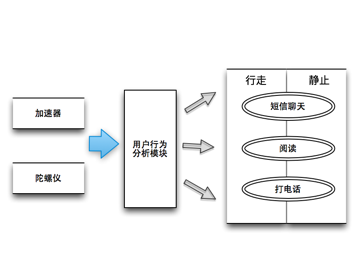
\includegraphics[width=4in]{walkstate}
  \caption{用户行为感知模块工作示意图}
  \label{fig:walkstate}
\end{figure}


\subsection{噪声属性分析与分类模块}

噪声属性分析模块即轻量特征分析模块。该模块的优势是响应迅速,该模块通过分析声音的音量变化特性、周期性和频谱特征曲线,最后基于规则对样本分类。规则及伪代码如下:

\begin{compactenum}
\item 分析音量变化特征,若不符合汽车噪声特点,排除,若符合,进入下一步。
\item 分析频谱,若是汽笛声,则得出结论有车靠近,并结束。若不是汽笛声,进入下一步。
\item 分析频谱特征曲线分析并尝试提取周期性,若成功提取到频率逐渐增大的周期且特征曲线和汽车噪声频谱特征曲线相似,则得出有车靠近的结论,并结束。若只满足两者中的一项,则调用复杂特征分析模块,若两项都不满足,则得出结论没有汽车靠近,并结束。
\end{compactenum}

这种方法可以识别出大部分的汽车靠近的样本,但有一部分无法识别。其无法识别的样本表现为无明显周期性或频谱特征曲线与基准曲线相关性较差。分类模块的设计就是为了识别这一部分样本。

分类模块即复杂特征分析模块。该模块基于机器学习中的K近邻算法对样本进行分类,优势是分类准确率高,但存在计算耗时的缺点。如果对每个样本都采用K近邻分类会严重拖慢系统的响应速度,因此,只有当轻量特征分析模块无法确定结果时才将样本转发给复杂特征分析模块。

两模块相互协作,共同保证了系统了准确率和较低的响应时间,模块协作的伪代码如下:

\begin{code}
//伪代码
Whille isWalking && usingPhone:
    Buffer <- AudioRecoder.read()
    if(result = ExtractSimpleFeature(Buffer))
        //如果轻量特征模块得出结论,则输出
        print result.value
        continue
    else
        //如果轻量特征分析模块无法得出结论,则调用复杂特征分析模块。
        result = KnnClassification(Buffer)
        print result.value

\end{code}



\section{性能评估}

\subsection{模块性能评估}
模块性能测试的目的是评估各模块对系统性能的作用。性能评估指标包括能耗,响应时间和识别率。实验者同时携带4部同类型智能手机(手机型号,初始电量,安装软件均相同),模拟包括上课,吃饭,校园内散步等活动在内的10小时日常生活。其中3部手机分别模拟关闭三模块中的一个模块,另外1部则模拟开启全部模块。共进行三组实验,结果如表~\ref{tab:closeA}、表~\ref{tab:closeB}、表~\ref{tab:closeC}和表~\ref{tab:closeNothing}所示。其中,耗电数据由系统电量统计软件得出,表示占手机电池总量的百分比;响应时间指从检测周期开始到得出检测结论所耗时间;识别率表示正确识别数占实际车辆数的百分比。


\begin{table}[htb]
\centering
\noindent\begin{minipage}{0.6\linewidth}
\centering
\caption[模块评估结果一]{关闭用户行为分析模块的结果}
\label{tab:closeA}
\begin{tabularx}{\linewidth}{cccc}
\toprule
& {\hei 耗电} & {\hei 平均响应时间} & {\hei 识别率} \\
\midrule
第一组 &  &  &  \\ 
第二组 &  &  &  \\ 
第三组 &  &  &  \\ 
平均 &  &  &  \\ 
\bottomrule
\end{tabularx}
\end{minipage}

\begin{minipage}{0.6\linewidth}
\centering
\caption[模块评估结果二]{关闭轻量特征分析模块的结果}
\label{tab:closeB}
\begin{tabularx}{\linewidth}{cccc}
\toprule
& {\hei 耗电} & {\hei 平均响应时间} & {\hei 识别率} \\
\midrule
第一组 &  &  &  \\ 
第二组 &  &  &  \\ 
第三组 &  &  &  \\ 
平均 &  &  &  \\ 
\bottomrule
\end{tabularx}
\end{minipage}

\begin{minipage}{0.6\linewidth}
\centering
\caption[模块评估结果三]{关闭复杂特征分析模块的结果}
\label{tab:closeC}
\begin{tabularx}{\linewidth}{cccc}
\toprule
& {\hei 耗电} & {\hei 平均响应时间} & {\hei 识别率} \\
\midrule
第一组 &  &  &  \\ 
第二组 &  &  &  \\ 
第三组 &  &  &  \\ 
平均 &  &  &  \\ 
\bottomrule
\end{tabularx}
\end{minipage}

\begin{minipage}{0.6\linewidth}
\centering
\caption[模块评估结果四]{三模块全部开启的结果}
\label{tab:closeNothing}
\begin{tabularx}{\linewidth}{cccc}
\toprule
& {\hei 耗电} & {\hei 平均响应时间} & {\hei 识别率} \\
\midrule
第一组 &  &  &  \\ 
第二组 &  &  &  \\ 
第三组 &  &  &  \\ 
平均 &  &  &  \\ 
\bottomrule
\end{tabularx}
\end{minipage}
\end{table}


实验结果表明,不开启用户行为分析模块,而是保持麦克风长时开启时,10小时平均耗电量为31\%,开启该模块后10小时平均耗电量仅为5\%,该模块的设计有效节约了手机电量;不开启轻量特征分析模块时,每一轮检测都交由复杂特征分析模块,平均响应时间为0.06 s,增加了轻量特征分析以后,平均响应缩短至0.017 s,响应速度大幅提升;不开启复杂特征分析模块时,车辆靠近情景的正确识别率只有84.74\%,增加了该模块后,识别率提高至94.5\%,提升效果明显。


\subsection{环境对性能的影响}
时间地点的影响

这部分实验作者选取了校园内的三条单车道单行线,并在每个地点进行了早中晚三个时间段的实验。地点a较偏僻,背景噪声单一;地点b为靠近校门口的交通枢纽早高峰和中午车辆和行人较多;地点c靠近火车道,实验过程中不定期有火车经过产生的噪声。三个地点共九组实验的正确识别率如图~\ref{fig:audioresult1}所示。
结果表明系统在同一地点的识别率会随时间变化,表现为晚上的识别率最高,中午的识别率最低。这是因为晚上背景噪声最小,而中午噪声最大。在同一时间段,不同地点,由于其背景噪声种类不同,识别率也有所不同。地点b和地点c由于有行人噪声和火车噪声,其整体识别率要差于地点a。

\begin{figure}[htbp] % use float package if you want it here
  \centering
  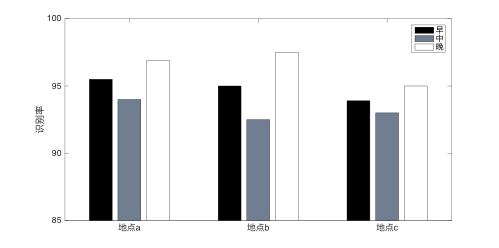
\includegraphics[width=4in]{audioresult1}
  \caption{时间地点对车辆识别率低影响图}
  \label{fig:audioresult1}
\end{figure}

车道数量的影响
这部分实验选取了五个具有不同车道数量的路段。实验者模拟正常行人在路边行走和横穿马路的行为,每个路段各进行3组实验。平均正确识别率随车道数量的变化如图~\ref{fig:audioresult2}所示。
从图~\ref{fig:audioresult2}可以看出,随着车道数量的增加系统对正在靠近的危险车辆识别率会有所降低。这是由于随着车道数量的增多,车流增大,周围环境中的噪声也随之变的嘈杂,影响了系统对车辆的检测。在常见的4车道,系统识别率可以保持在85\%以上,可以说系统具有了一定的鲁棒性,但仍有改进空间。

\begin{figure}[htbp] % use float package if you want it here
  \centering
  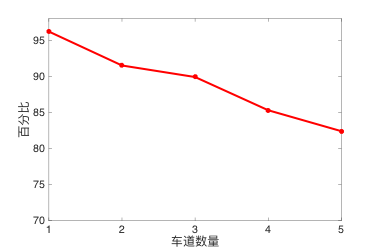
\includegraphics[width=4in]{audioresult2}
  \caption{车道数量对识别率的影响}
  \label{fig:audioresult2}
\end{figure}

\section{本章小结}

本章详细介绍了一个利用智能手机帮助“低头族”感知危险的安全辅助方法。通过手机内置的麦克风收集行人周围的声音数据,从中提取出和汽车靠近有关的信息,并向正在低头使用手机的行人发出相应警告。相比于现有基于手机摄像头的解决方案,此种方法更加易用,感知范围更大,其多模块的设计更是大大降低了耗电量,且提高了识别率。针对系统的性能评估,作者进行了大量实验,结果表明环境对系统性能的影响有限,系统对环境具有一定容忍性,可以起到安全辅助的效果。


% \subsection{感知需求及目标}

% 用户周围有无车辆

% 车辆行驶状态

% \section{现有工作(基于摄像头的)}

% \section{声音感知车辆原理}
% 正文内容

% \section{系统设计}
% 正文内容
% \subsection{音频数据获取}

% \subsection{音频信号的处理方法}
% 正文内容
% \subsection{车辆噪声的时频特征分析}

% \subsection{基于机器学习的噪声来源分类}
% 正文内容

% \section{性能评估}
% 正文内容
% \subsection{实验设计}
% \subsection{结果与分析}

% \section{本章小结}